
\section{Der Prim-Algorithmus}


\begin{bem}
In diesem Abschnitt sei $G=(V,E)$ ein (ungerichteter) Graph und $w : E \to \R$ eine \textbf{Gewichtsfunktion} auf seinen Kanten.
Das hei\ss t, jeder Kante $\{u,v\} \in E$ wird eine Zahl (ihr \textbf{Gewicht}) $w(u,v) \in \R$ zugeordnet.
Das Tripel $G=(V,E,w)$ hei\ss t dann \textbf{gewichteter Graph}.
Wir nehmen im Folgenden stets an, dass der Graph~$G$ \underline{zusammenhängend} ist.

Um die Gewichtsfunktion in die Adjazenzliste von $G$ aufzunehmen, kann man die Nachbarn $N[u]$ eines Knotens $u \in V$ zum Beispiel als Paare $(v,w(u,v)) \in V \times \R$ führen.
\end{bem}

\begin{defn}
Sei $G=(V,E,w)$ ein gewichteter Graph.
Ein Baum $T=(V',E')$ heißt \textbf{Spannbaum} von~$G$, falls $V=V'$ und $E' \subseteq E$ gelten.
Für jeden Teilgraphen $G' = (V',E')$ von~$G$ definieren wir sein \textbf{Gewicht} als
\[
w(G') := \sum_{e \in E'} w(e).
\]
%
Ein Spannbaum $T=(V,E')$ von~$G$ heißt \textbf{minimaler Spannbaum}, wenn~$T$ unter allen Spannbäumen von~$G$ minimales Gewicht hat.
\end{defn} 


\begin{bsp}
Jeder Breitensuchbaum und jeder Tiefensuchbaum ist ein Spannbaum.
Im Allgemeinen sind diese Spannbäume aber keine \underline{minimalen} Spannbäume:\\[1em]

\hfill
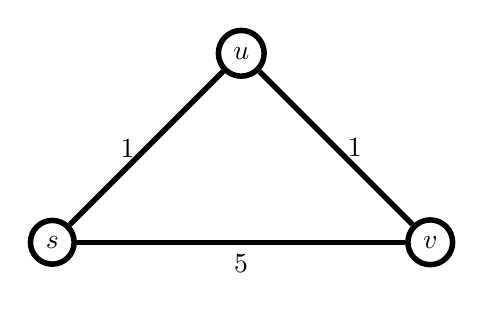
\begin{tikzpicture}[line width=2,scale=1.2]
	 \node[circle,draw=black] (s) at (0,0) {$s$};
	 \node[circle,draw=black] (u) at (2,2) {$u$};
	 \node[circle,draw=black] (v) at (4,0) {$v$};
	 \draw[-] (s) edge node[midway,left]{$1$} (u);
	 \draw[-] (u) edge node[midway,right]{$1$} (v);
	 \draw[-] (v) edge node[midway,below]{$5$} (s);
\end{tikzpicture}
\hfill\,


\end{bsp}

\begin{prop}
Sei $G=(V,E,w)$ ein gewichteter Graph mit paarweise verschiedenen Kantengewichten, das hei\ss t, für je zwei Kanten $\{u,v\} \neq \{r,s\}$ von~$G$ gilt $w(u,v) \neq w(r,s)$.
Dann gibt es genau einen minimalen Spannbaum in~$G$.
\end{prop}
\begin{proof}
Angenommen, es gibt zwei verschiedene minimale Spannbäume $S$ und $T$ von~$G$.
Dann gibt es mindestens eine Kante $e \in E$, die in $S \setminus T$ oder in $T \setminus S$ liegt.
Sei $e_1$ unter allen solchen Kanten, die Kante kleinsten Gewichts, also $w(e_1) < w(e)$, für alle Kanten $e \in S \setminus T \cup T \setminus S$.
Ohne Einschränkung sei $e_1 \in S \setminus T$. (Die Kante $e_1$ ist insbesondere eindeutig.)

Da $T$ ein Spannbaum ist, enthält der Teilgraph $T \cup \{e_1\}$ einen Kreis $C$, der wiederum die Kante $e_1$ enthält.
Der Spannbaum~$S$ ist als Baum ein kreisfreier Graph, und somit gibt es eine Kante $e_2 \in C \setminus S$, und $e_2$ gehört zu~$T$.
Nach Annahme an die Kante~$e_1$, gilt $w(e_2) > w(e_1)$.

\condclearpage

Wir betrachten den Graphen $T' := T \setminus \{e_2\} \cup \{e_1\}$.
Da~$C$ der einizige Kreis in $T \cup \{e_1\}$ ist, ist $T'$ kreisfrei und es ist $|E(T')| = |E(T)| = |V|-1$.
Somit ist $T'$ wiederum ein Spannbaum von~$G$ (siehe Übungszettel).
Weiterhin gilt
\[
w(T') = w(T) - w(e_2) + w(e_1) < w(T),
\]
was im Widerspruch dazu steht, dass $T$ als minimaler Spannbaum angenommen wurde.
\end{proof}

\begin{bem} 
Unser Ziel ist es, das \textbf{Problem des minimalen Spannbaums} möglichst effizient zu lösen:
\begin{center}
\textit{Gegeben ein zusammenhängender gewichteter Graph~$G=(V,E,w)$,\\ finde einen minimalen Spannbaum von~$G$.}
\end{center}
%
\noindent Das Bestimmen eines \underline{minimalen} Spannbaums ist in verschiedenen Problemen praxisrelevant:
%
\begin{itemize}
 \item Verlegen von Glasfaserkabeln (Gewicht einer Verbindung als Funktion von Länge, Tiefe, Bodenbeschaffenheit, etc.)
% \item Bei elektronischen Schaltkreisen will man eine Menge von Kontakten verdrahten, um diese auf das gleiche Potenzial zu legen.
 \item \emph{Spanning tree protocol} (Übersendung von Paketen in einem Netzwerk).
 \item Approximationslösung für das \emph{Problem der Handlungsreisenden}.
 \item Generieren von \emph{Labyrinthen} für Spiele (siehe zB.~\url{https://de.wikipedia.org/wiki/Datei:MAZE_30x20_Prim.ogv}).
\end{itemize}
Wir legen Ihnen nahe, sich mit diesen Anwendungen selbst etwas vertraut zu machen und nachzuvollziehen, inwiefern das Finden eines minimalen Spannbaums in jedem dieser Beispiele von Nutzen ist.
\end{bem} 

\begin{thm}[Cayley]
Der vollständige Graph $K_n$ auf $n$ Knoten hat $n^{n-2}$ Spannbäume.
\end{thm}
Als Folge ist der naive algorithmische Ansatz des Enumerierens aller Spannbäume nicht effizient.


\begin{bem}
Sind alle Kantengewichte in $G=(V,E,w)$ positiv, also $w(u,v) > 0$, für alle $\{u,v\} \in E$, so ist das Problem des minimalen Spannbaums äquivalent zum Problem der Bestimmung eines zusammenhängenden Teilgraphen $G'= (V',E')$ von $G$ mit $V=V'$ und dem kleinsten Gewicht.
\end{bem}

\begin{bem} 
In der Literatur gibt es eine ganze Reihe von Algorithmen zur Lösung des Problems des minimalen Spannbaums.
Wir diskutieren hier den sogennanten \textbf{Prim-Algorithmus} der im Jahr 1957 in einer Arbeit von Robert C.~Prim erschien und zwei Jahre später von Dijkstra neu beschrieben wurde.
Beiden Autoren (und allgemein der westlichen Forschergemeinschaft) war anscheinend die Arbeit von Vojt\v{e}ch Jarn\'{i}k aus dem Jahr 1930 nicht bekannt, der die Vorgehensweise bereits lange zuvor diskutierte.
\end{bem} 

\begin{bem}
\underline{Grundidee des Prim-Algorithmus:}
Der Algorithmus basiert auf der einfachen Idee einen Spannbaum sukzessive \glqq von Null auf\grqq\ durch das Hinzufügen von Kanten kleinstmöglichen Gewichtes wachsen zu lassen.
Genauer gesagt starten wir mit einem Startbaum~$T_0$, der aus einem beliebigen Knoten~$s$ von~$G$ besteht.
Diesen erweitern wir dann durch eine zu~$s$ adjazente Kante kleinsten Gewichtes zu dem Teilbaum~$T_1$.
Im nächsten Schritt wählen wir wieder eine Kante kleinsten Gewichtes unter den verbleibenden Kanten in~$G$ aus, die zu $T_1$ hinzugefügt werden kann und dabei die Baumeigenschaft erhält.
Wir bekommen dadurch den Teilbaum~$T_2$, der nun aus zwei Kanten besteht.
Führen wir dies Schritt für Schritt weiter gelangen wir zu einem Teilbaum~$T_{|V|-1}$ der aus $|V|-1$ Kanten besteht und ein Spannbaum von~$G$ ist.
Der Clou ist nun, dass dieser Spannbaum minimales Gewicht unter allen Spannbäumen von~$G$ hat.
\end{bem} 


\begin{bsp}
\label{bsp:prim}
Gegeben sei der folgende gewichtete zusammenhängende Graph:
%
\begin{center}
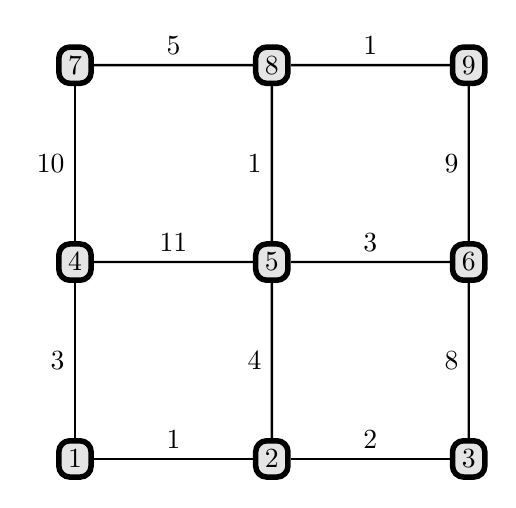
\begin{tikzpicture}[line width=2,scale=2.5]
\tikzstyle{V}=
 =[
 fill=gray!20, rounded corners, draw=black
 ]

\node[V] (1) at (0,0) {$1$};
\node[V] (2) at (1,0) {$2$};
\node[V] (3) at (2,0) {$3$};
\node[V] (4) at (0,1) {$4$};
\node[V] (5) at (1,1) {$5$};
\node[V] (6) at (2,1) {$6$};
\node[V] (7) at (0,2) {$7$};
\node[V] (8) at (1,2) {$8$};
\node[V] (9) at (2,2) {$9$};
	
\draw[line width=0.3mm] 
 (1) edge node[midway,above]{$1$} (2)  
 (2) edge node[midway,above]{$2$} (3) 
 (4) edge node[midway,above]{$11$} (5) 
 (5) edge node[midway,above]{$3$} (6) 
 (7) edge node[midway,above]{$5$} (8)
 (8) edge node[midway,above]{$1$} (9)
 (1) edge node[midway,left]{$3$} (4)
 (2) edge node[midway,left]{$4$} (5)
 (3) edge node[midway,left]{$8$} (6)
 (4) edge node[midway,left]{$10$} (7)
 (5) edge node[midway,left]{$1$} (8)
 (6) edge node[midway,left]{$9$} (9)
;
\end{tikzpicture}	
\end{center}
%
Beginnend vom Startknoten~$s=1$ illustrieren wir die Vorgehensweise des Prim-Algorithmus.
In jedem Graphen der folgenden Sequenz markieren wir den aktuellen Teilbaum~$T_i$ in rot und die in Frage kommenden Kanten für die Erweiterung zum Teilbaum $T_{i+1}$ in grün:
\begin{center}
\hfill
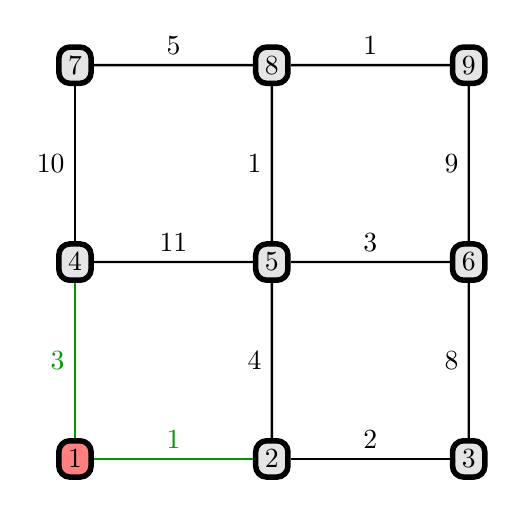
\begin{tikzpicture}[line width=2,scale=2.5]
\tikzstyle{V}=
 =[
 fill=gray!20, rounded corners, draw=black
 ]
\tikzstyle{R}=
 =[
 fill=red!50, rounded corners, draw=black
 ]

\node[R] (1) at (0,0) {$1$};
\node[V] (2) at (1,0) {$2$};
\node[V] (3) at (2,0) {$3$};
\node[V] (4) at (0,1) {$4$};
\node[V] (5) at (1,1) {$5$};
\node[V] (6) at (2,1) {$6$};
\node[V] (7) at (0,2) {$7$};
\node[V] (8) at (1,2) {$8$};
\node[V] (9) at (2,2) {$9$};
	
\draw[line width=0.3mm] 
 (1) edge[green!60!black] node[midway,above]{$1$} (2)  
 (2) edge node[midway,above]{$2$} (3) 
 (4) edge node[midway,above]{$11$} (5) 
 (5) edge node[midway,above]{$3$} (6) 
 (7) edge node[midway,above]{$5$} (8)
 (8) edge node[midway,above]{$1$} (9)
 (1) edge[green!60!black] node[midway,left]{$3$} (4)
 (2) edge node[midway,left]{$4$} (5)
 (3) edge node[midway,left]{$8$} (6)
 (4) edge node[midway,left]{$10$} (7)
 (5) edge node[midway,left]{$1$} (8)
 (6) edge node[midway,left]{$9$} (9)
;
\end{tikzpicture}	
\hfill
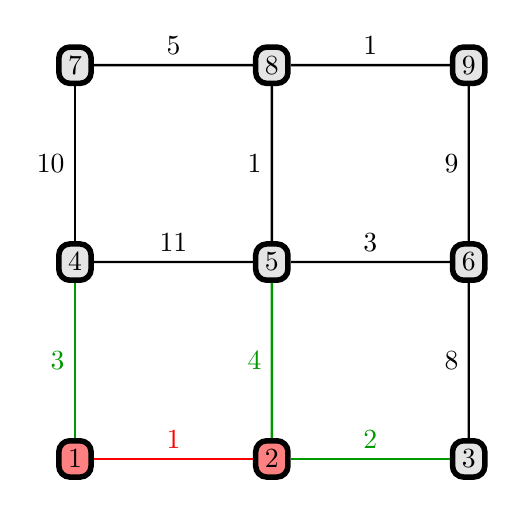
\begin{tikzpicture}[line width=2,scale=2.5]
\tikzstyle{V}=
 =[
 fill=gray!20, rounded corners, draw=black
 ]
\tikzstyle{R}=
 =[
 fill=red!50, rounded corners, draw=black
 ]

\node[R] (1) at (0,0) {$1$};
\node[R] (2) at (1,0) {$2$};
\node[V] (3) at (2,0) {$3$};
\node[V] (4) at (0,1) {$4$};
\node[V] (5) at (1,1) {$5$};
\node[V] (6) at (2,1) {$6$};
\node[V] (7) at (0,2) {$7$};
\node[V] (8) at (1,2) {$8$};
\node[V] (9) at (2,2) {$9$};
	
\draw[line width=0.3mm] 
 (1) edge[red] node[midway,above]{$1$} (2)  
 (2) edge[green!60!black] node[midway,above]{$2$} (3) 
 (4) edge node[midway,above]{$11$} (5) 
 (5) edge node[midway,above]{$3$} (6) 
 (7) edge node[midway,above]{$5$} (8)
 (8) edge node[midway,above]{$1$} (9)
 (1) edge[green!60!black] node[midway,left]{$3$} (4)
 (2) edge[green!60!black] node[midway,left]{$4$} (5)
 (3) edge node[midway,left]{$8$} (6)
 (4) edge node[midway,left]{$10$} (7)
 (5) edge node[midway,left]{$1$} (8)
 (6) edge node[midway,left]{$9$} (9)
;
\end{tikzpicture}	
\hfill\,
\end{center}
\begin{center}
\hfill
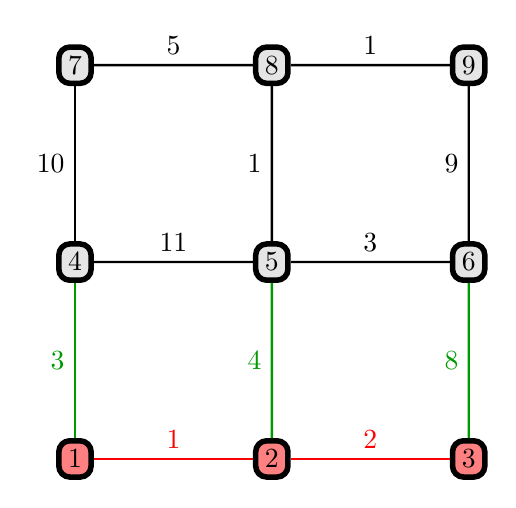
\begin{tikzpicture}[line width=2,scale=2.5]
\tikzstyle{V}=
 =[
 fill=gray!20, rounded corners, draw=black
 ]
\tikzstyle{R}=
 =[
 fill=red!50, rounded corners, draw=black
 ]

\node[R] (1) at (0,0) {$1$};
\node[R] (2) at (1,0) {$2$};
\node[R] (3) at (2,0) {$3$};
\node[V] (4) at (0,1) {$4$};
\node[V] (5) at (1,1) {$5$};
\node[V] (6) at (2,1) {$6$};
\node[V] (7) at (0,2) {$7$};
\node[V] (8) at (1,2) {$8$};
\node[V] (9) at (2,2) {$9$};
	
\draw[line width=0.3mm] 
 (1) edge[red] node[midway,above]{$1$} (2)  
 (2) edge[red] node[midway,above]{$2$} (3) 
 (4) edge node[midway,above]{$11$} (5) 
 (5) edge node[midway,above]{$3$} (6) 
 (7) edge node[midway,above]{$5$} (8)
 (8) edge node[midway,above]{$1$} (9)
 (1) edge[green!60!black] node[midway,left]{$3$} (4)
 (2) edge[green!60!black] node[midway,left]{$4$} (5)
 (3) edge[green!60!black] node[midway,left]{$8$} (6)
 (4) edge node[midway,left]{$10$} (7)
 (5) edge node[midway,left]{$1$} (8)
 (6) edge node[midway,left]{$9$} (9)
;
\end{tikzpicture}	
\hfill
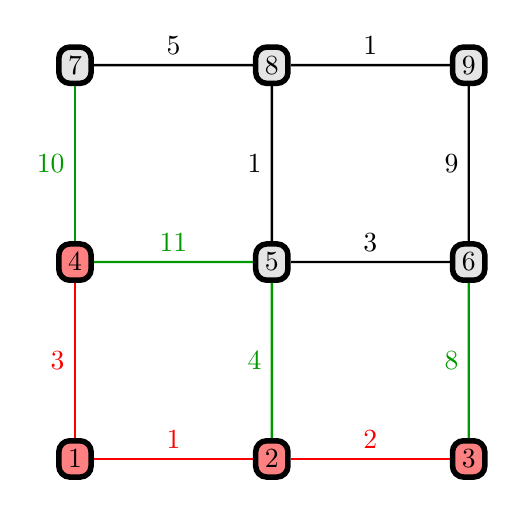
\begin{tikzpicture}[line width=2,scale=2.5]
\tikzstyle{V}=
 =[
 fill=gray!20, rounded corners, draw=black
 ]
\tikzstyle{R}=
 =[
 fill=red!50, rounded corners, draw=black
 ]

\node[R] (1) at (0,0) {$1$};
\node[R] (2) at (1,0) {$2$};
\node[R] (3) at (2,0) {$3$};
\node[R] (4) at (0,1) {$4$};
\node[V] (5) at (1,1) {$5$};
\node[V] (6) at (2,1) {$6$};
\node[V] (7) at (0,2) {$7$};
\node[V] (8) at (1,2) {$8$};
\node[V] (9) at (2,2) {$9$};
	
\draw[line width=0.3mm] 
 (1) edge[red] node[midway,above]{$1$} (2)  
 (2) edge[red] node[midway,above]{$2$} (3) 
 (4) edge[green!60!black] node[midway,above]{$11$} (5) 
 (5) edge node[midway,above]{$3$} (6) 
 (7) edge node[midway,above]{$5$} (8)
 (8) edge node[midway,above]{$1$} (9)
 (1) edge[red] node[midway,left]{$3$} (4)
 (2) edge[green!60!black] node[midway,left]{$4$} (5)
 (3) edge[green!60!black] node[midway,left]{$8$} (6)
 (4) edge[green!60!black] node[midway,left]{$10$} (7)
 (5) edge node[midway,left]{$1$} (8)
 (6) edge node[midway,left]{$9$} (9)
;
\end{tikzpicture}	
\hfill\,
\end{center}
\begin{center}
\hfill
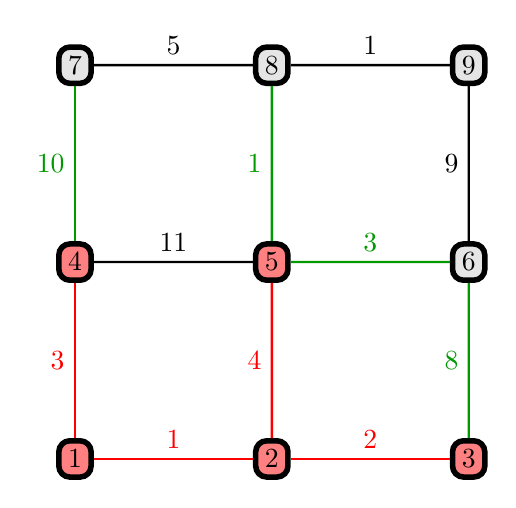
\begin{tikzpicture}[line width=2,scale=2.5]
\tikzstyle{V}=
 =[
 fill=gray!20, rounded corners, draw=black
 ]
\tikzstyle{R}=
 =[
 fill=red!50, rounded corners, draw=black
 ]

\node[R] (1) at (0,0) {$1$};
\node[R] (2) at (1,0) {$2$};
\node[R] (3) at (2,0) {$3$};
\node[R] (4) at (0,1) {$4$};
\node[R] (5) at (1,1) {$5$};
\node[V] (6) at (2,1) {$6$};
\node[V] (7) at (0,2) {$7$};
\node[V] (8) at (1,2) {$8$};
\node[V] (9) at (2,2) {$9$};
	
\draw[line width=0.3mm] 
 (1) edge[red] node[midway,above]{$1$} (2)  
 (2) edge[red] node[midway,above]{$2$} (3) 
 (4) edge node[midway,above]{$11$} (5) 
 (5) edge[green!60!black] node[midway,above]{$3$} (6) 
 (7) edge node[midway,above]{$5$} (8)
 (8) edge node[midway,above]{$1$} (9)
 (1) edge[red] node[midway,left]{$3$} (4)
 (2) edge[red] node[midway,left]{$4$} (5)
 (3) edge[green!60!black] node[midway,left]{$8$} (6)
 (4) edge[green!60!black] node[midway,left]{$10$} (7)
 (5) edge[green!60!black] node[midway,left]{$1$} (8)
 (6) edge node[midway,left]{$9$} (9)
;
\end{tikzpicture}	
\hfill
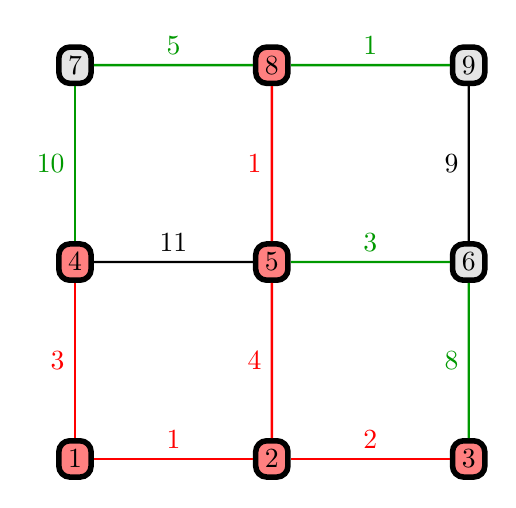
\begin{tikzpicture}[line width=2,scale=2.5]
\tikzstyle{V}=
 =[
 fill=gray!20, rounded corners, draw=black
 ]
\tikzstyle{R}=
 =[
 fill=red!50, rounded corners, draw=black
 ]

\node[R] (1) at (0,0) {$1$};
\node[R] (2) at (1,0) {$2$};
\node[R] (3) at (2,0) {$3$};
\node[R] (4) at (0,1) {$4$};
\node[R] (5) at (1,1) {$5$};
\node[V] (6) at (2,1) {$6$};
\node[V] (7) at (0,2) {$7$};
\node[R] (8) at (1,2) {$8$};
\node[V] (9) at (2,2) {$9$};
	
\draw[line width=0.3mm] 
 (1) edge[red] node[midway,above]{$1$} (2)  
 (2) edge[red] node[midway,above]{$2$} (3) 
 (4) edge node[midway,above]{$11$} (5) 
 (5) edge[green!60!black] node[midway,above]{$3$} (6) 
 (7) edge[green!60!black] node[midway,above]{$5$} (8)
 (8) edge[green!60!black] node[midway,above]{$1$} (9)
 (1) edge[red] node[midway,left]{$3$} (4)
 (2) edge[red] node[midway,left]{$4$} (5)
 (3) edge[green!60!black] node[midway,left]{$8$} (6)
 (4) edge[green!60!black] node[midway,left]{$10$} (7)
 (5) edge[red] node[midway,left]{$1$} (8)
 (6) edge node[midway,left]{$9$} (9)
;
\end{tikzpicture}	
\hfill\,
\end{center}
\begin{center}
\hfill
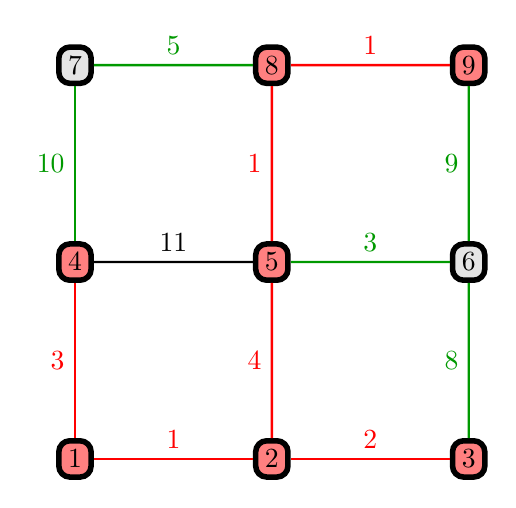
\begin{tikzpicture}[line width=2,scale=2.5]
\tikzstyle{V}=
 =[
 fill=gray!20, rounded corners, draw=black
 ]
\tikzstyle{R}=
 =[
 fill=red!50, rounded corners, draw=black
 ]

\node[R] (1) at (0,0) {$1$};
\node[R] (2) at (1,0) {$2$};
\node[R] (3) at (2,0) {$3$};
\node[R] (4) at (0,1) {$4$};
\node[R] (5) at (1,1) {$5$};
\node[V] (6) at (2,1) {$6$};
\node[V] (7) at (0,2) {$7$};
\node[R] (8) at (1,2) {$8$};
\node[R] (9) at (2,2) {$9$};
	
\draw[line width=0.3mm] 
 (1) edge[red] node[midway,above]{$1$} (2)  
 (2) edge[red] node[midway,above]{$2$} (3) 
 (4) edge node[midway,above]{$11$} (5) 
 (5) edge[green!60!black] node[midway,above]{$3$} (6) 
 (7) edge[green!60!black] node[midway,above]{$5$} (8)
 (8) edge[red] node[midway,above]{$1$} (9)
 (1) edge[red] node[midway,left]{$3$} (4)
 (2) edge[red] node[midway,left]{$4$} (5)
 (3) edge[green!60!black] node[midway,left]{$8$} (6)
 (4) edge[green!60!black] node[midway,left]{$10$} (7)
 (5) edge[red] node[midway,left]{$1$} (8)
 (6) edge[green!60!black] node[midway,left]{$9$} (9)
;
\end{tikzpicture}	
\hfill
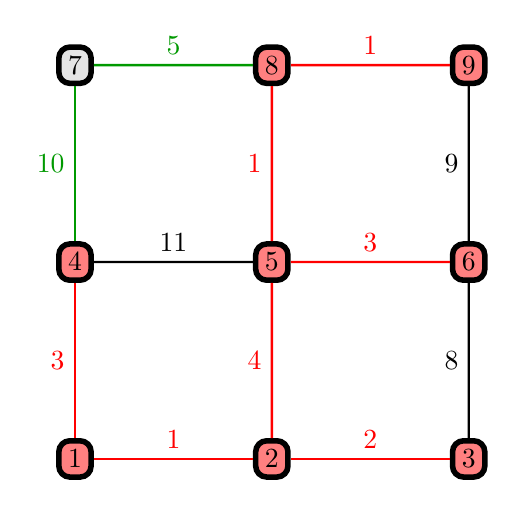
\begin{tikzpicture}[line width=2,scale=2.5]
\tikzstyle{V}=
 =[
 fill=gray!20, rounded corners, draw=black
 ]
\tikzstyle{R}=
 =[
 fill=red!50, rounded corners, draw=black
 ]

\node[R] (1) at (0,0) {$1$};
\node[R] (2) at (1,0) {$2$};
\node[R] (3) at (2,0) {$3$};
\node[R] (4) at (0,1) {$4$};
\node[R] (5) at (1,1) {$5$};
\node[R] (6) at (2,1) {$6$};
\node[V] (7) at (0,2) {$7$};
\node[R] (8) at (1,2) {$8$};
\node[R] (9) at (2,2) {$9$};
	
\draw[line width=0.3mm] 
 (1) edge[red] node[midway,above]{$1$} (2)  
 (2) edge[red] node[midway,above]{$2$} (3) 
 (4) edge node[midway,above]{$11$} (5) 
 (5) edge[red] node[midway,above]{$3$} (6) 
 (7) edge[green!60!black] node[midway,above]{$5$} (8)
 (8) edge[red] node[midway,above]{$1$} (9)
 (1) edge[red] node[midway,left]{$3$} (4)
 (2) edge[red] node[midway,left]{$4$} (5)
 (3) edge node[midway,left]{$8$} (6)
 (4) edge[green!60!black] node[midway,left]{$10$} (7)
 (5) edge[red] node[midway,left]{$1$} (8)
 (6) edge node[midway,left]{$9$} (9)
;
\end{tikzpicture}	
\hfill\,
\end{center}
\begin{center}
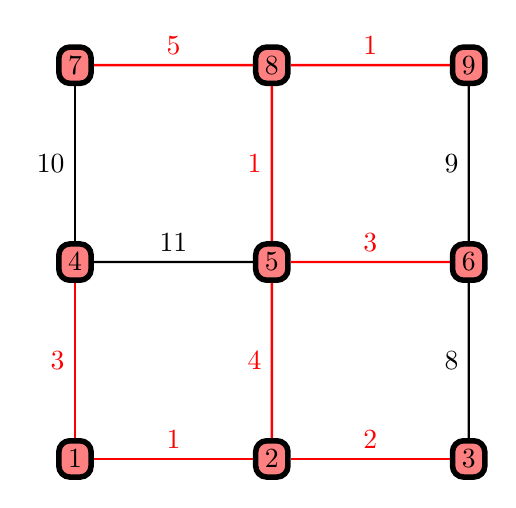
\begin{tikzpicture}[line width=2,scale=2.5]
\tikzstyle{V}=
 =[
 fill=gray!20, rounded corners, draw=black
 ]
\tikzstyle{R}=
 =[
 fill=red!50, rounded corners, draw=black
 ]

\node[R] (1) at (0,0) {$1$};
\node[R] (2) at (1,0) {$2$};
\node[R] (3) at (2,0) {$3$};
\node[R] (4) at (0,1) {$4$};
\node[R] (5) at (1,1) {$5$};
\node[R] (6) at (2,1) {$6$};
\node[R] (7) at (0,2) {$7$};
\node[R] (8) at (1,2) {$8$};
\node[R] (9) at (2,2) {$9$};
	
\draw[line width=0.3mm] 
 (1) edge[red] node[midway,above]{$1$} (2)  
 (2) edge[red] node[midway,above]{$2$} (3) 
 (4) edge node[midway,above]{$11$} (5) 
 (5) edge[red] node[midway,above]{$3$} (6) 
 (7) edge[red] node[midway,above]{$5$} (8)
 (8) edge[red] node[midway,above]{$1$} (9)
 (1) edge[red] node[midway,left]{$3$} (4)
 (2) edge[red] node[midway,left]{$4$} (5)
 (3) edge node[midway,left]{$8$} (6)
 (4) edge node[midway,left]{$10$} (7)
 (5) edge[red] node[midway,left]{$1$} (8)
 (6) edge node[midway,left]{$9$} (9)
;
\end{tikzpicture}	
\end{center}
\end{bsp}

\begin{bem}
Für die Umsetzung dieser simplen Idee benötigen wir eine weitere Datenstruktur, die das sukzessive Auswählen der noch verfügbaren Kante kleinstmöglichen Gewichts erlaubt.
\end{bem}

\begin{defn}
	Seien $X$ und $K$ Mengen. 
	Wir definieren die \textbf{Prioritätswarteschlange}~$S$ bzgl. $X$ und $K$ als eine Datenstruktur zur Speicherung und Verwaltung von Wert-Schlüssel-Paaren $(x,k)$ mit $x \in X$ und $k \in K$.
	 
	 Die folgenden Grundoperationen stehen dabei zur Verfügung: 
%
\begin{itemize}
 \item $\cc{Einf\"ugen}(S,(x,k))$
 
 Fügt das Element $(x,k)$ zur Menge $S$ hinzu.

 \item $\cc{Entfernen}(S,(x,k))$
 
 Entfernt das Element~$(x,k)$ aus $S$.

 \item $\cc{Minimum}(S)$
 
 Gibt das Element von $S$ mit dem kleinsten Schlüssel zurück.
 
 \item $\cc{Minimum-Entfernen}(S)$
 
 Entfernt das Element mit dem kleinsten Schlüssel aus~$S$ und gibt dieses zurück.

 \item $\cc{Schl\"u{\ss}el-\"Andern}(S,(x,k),\ell)$
 
 Ändert den Schlüssel des in~$S$ enthaltenen Elements $(x,k)$ auf den Wert~$\ell$.
 
 (Die Änderung ist eine redundante Operation, die der Entfernung von $(x,k)$ und dem Einfügen von $(x,\ell)$ entspricht.) 
\end{itemize}

%	\begin{enuma}
%			\item Initialisierung: Erzeugung einer leeren Prioritätschlange $S$ zur Speicherung von höchstens $n \in \N$ Elementen.
%			\item Aufnahme eines neuen Wert-Schlüssel Paares $(x,k)$ in $S$. 
%			\item Entfernung und Rückgabe eines Paares $(x,k)$ für, welches der Schlüssel $k$ innerhalb von $S$ minimal ist. 
%			\item Änderung des Schlüssels für ein Paar $(x,k)$. (Die Änderung ist eine redundante Operation, die der Enfernung von $x$ und der Aufnahme von $y$ entspricht.) 
%	\end{enuma}
%
\noindent Hierbei wird vorausgesetzt, dass die Schlüssel $k$ aus einer zugrundeliegenden totalgeordneten Menge $(K,\preceq)$ gewählt werden, sodass man je zwei Schlüssel $k,k'$ mit Hilfe der Ordnungsrelation~$\preceq$ vergleichen kann. (In vielen praktischen Situationen reicht es als $(K,\le)$ die totalgeordnete Menge $(\Z,\le)$ der ganzen Zahlen zu wählen.)
\end{defn} 


\begin{bem}
	Bei einer direkten/naiven Umsetzung der Prioritätswarteschlangen auf der Basis von Arrays mit sequentieller Suche beträgt der Aufwand zur Aufnahme eines Elements $\Theta(1)$ Elementaroperationen, während man für die Entfernung eines Elements im Worst-Case $\Theta(n)$ Elementaroperationen benötigt. Wenn man also $n$ Elemente bei einer solchen Umsetzung in die Schlange hinzufügt und dann all diese Elemente wieder entfernt, so hat man im Worst-Case den Gesamtaufwand von $\Theta(n^2)$ an Elementaroperationen bei einem solchen Ablauf.
\end{bem} 

\begin{bem}
	Mit Hilfe von sogenannten Heaps lässt sich die Prioritätswarteschlange so umsetzen, dass für die Durchführung einer jeden Grundoperation nur $O(\log n)$ Elementaroperationen benötigt werden. Mehr dazu im Modul \glqq Algorithmieren und Programmieren\grqq. Man nennt solche Prioritätswarteschlangen dann \textbf{Heap-basiert}.
\end{bem} 


\begin{bem}
Die Umsetzung der Grundidee des Prim-Algorithmus erfolgt nun entlang des nachfolgenden Pseudocodes mit den folgenden Attributen:
\begin{itemize}
 \item $Q$ ist eine Prioritätswarteschlange auf der Knotenmenge $V$
 \item Die Vorgängerabbildung ist wieder durch das Attribut~$\pi[v]$, für $v \in V$, beschrieben.
 \item Der aktuelle Teilbaum $(V',E')$, der nach obiger Idee sukzessive zu einem minimalen Spannbaum erweitert wird, hat zu jedem Zeitpunkt der Ausführung die Knotenmenge $V' = V \setminus Q$ und die Kantenmenge $E' = \left\{\{\pi[v],v\} : v \in V' \setminus \{s\}\right\}$.
 \item Das Attribut $\ell[v]$ für jeden Knoten $v \in V$ fungiert als Schlüssel für die Elemente in $Q$. Dabei ist für alle Knoten~$v \in Q$ mit $\pi[v] \neq \cc{nil}$ das Attribut $\ell[v] < \infty$ und entspricht dem Gewicht der Kante~$\{\pi[v],v\}$.
Diese Kante ist eine Kante mit aktuell kleinstem Gewicht, die den Knoten~$v$ mit dem aktuellen Teilbaum $(V',E')$ verbindet.
\end{itemize}


\begin{algorithm}[H]
\caption{$\cc{Prim}(G)$}
\begin{algorithmic}[1]
 \STATE Ein beliebiges $s \in V$ fixieren.
 \STATE\COMMENT{Initialisierung}
 \FOR{$v \in V$}
  \STATE $\ell[v] := \infty$
  \STATE $\pi[v] := \cc{nil}$
 \ENDFOR
 \STATE $\ell[s] := 0$
 \STATE $Q := $ Prioritätswarteschlange mit $\ell$ als Schlüssel, die alle Knoten $v \in V$ enthält.
 \STATE\COMMENT{Iteratives Aktualisieren der Kanten}
 \WHILE{$Q \neq \emptyset$}
  \STATE $u := \cc{Minimum-Entfernen}(Q)$ 
  \FOR{$v \in N[u]$}
   \STATE $\cc{Prim-Update}(u,v)$
  \ENDFOR
 \ENDWHILE
\end{algorithmic}
\end{algorithm}

Die Hilfsprozedur $\cc{Prim-Update}(u,v)$ ist wie folgt umgesetzt:

\begin{algorithm}[H]
	\caption{$\cc{Prim-Update}(u,v)$}
	\begin{algorithmic}[1]
		\IF{$v \in Q$ und $w(u,v) < \ell[v]$}
		\STATE $\ell[v]:=w(u,v)$
		\STATE $\pi[v] := u$
		\ENDIF
	\end{algorithmic}
\end{algorithm}

Damit in dieser Hilfsprozedur der Test \glqq Ist $v \in Q$?\grqq\ schnell, das heißt, in konstanter Zeit, durchgeführt werden kann, verwalten wir ein Array, das für jeden Knoten $v \in V$ notiert, ob der Knoten aktuell in~$Q$ enthalten ist oder nicht. So ein Array entspricht dem Array mit Farbattributen in der Breiten- oder Tiefensuche. 
\end{bem}

\begin{aufg}
Verfolgen Sie die Arbeitsweise von $\cc{Prim}(G)$ anhand der Dynamiken der involvierten Objekte~$Q$, $\ell$ und~$\pi$ auf dem gewichteten Graphen in Beispiel~\ref{bsp:prim}.
\end{aufg}

\begin{bem}
Nach erfolgter Ausführung des Prim-Algorithmus entspricht der letzte aktuelle Teilbaum $(V',E')$ dem \textbf{Vorgängerteilgraphen} $G_\pi := (V,E_\pi)$ von~$G$ mit Kantenmenge
\[
E_\pi := \setcond{ \{\pi[v],v\}}{v \in V \setminus \{s\}}.
\]
Wie oben bereits erwähnt stellt sich heraus, dass dieser Vorgängerteilgraph tatsächlich ein minimaler Spannbaum von~$G$ ist:
\end{bem} 

\begin{thm}
\label{thm:prim-korrektheit}
Sei $G=(V,E,w)$ ein zusammenhängender gewichteter Graph, der durch eine Adjazenzliste gegeben ist. 
Der Algorithmus $\cc{Prim}(G)$ löst das Problem des minimalen Spannbaums korrekt, das heißt, der Vorgängerteilgraph~$G_\pi$ ist ein minimaler Spannbaum von~$G$.

Ist die Prioritätswarteschlange auf der Basis von Heaps umgesetzt, so beträgt die Laufzeit des Verfahrens $O(|E| \log |V|)$. 
\end{thm}

\begin{proof}
Schauen wir zuerst auf die Laufzeit von $\cc{Prim}(G)$.
Die Initialisierung verläuft in Zeit $\Theta(|V|)$.
Beachten Sie dabei lediglich, dass die Prioritätswarteschlange~$Q$ in linearer Zeit initialisert werden kann, da die Schlüssel für die Knoten $v \neq s$ alle gleich $\infty$ sind.
Die Initialisierung kann also durch ein Array $[s,v_1,\ldots,v_k]$ erfolgen, wobei $v_1,\ldots,v_k$ eine beliebige Anordnung der Knoten in $V \setminus \{s\}$ ist.

Nach erfolgter Initialisierung wird die \texttt{while}-Schleife exakt $|V|$ Mal aufgerufen, ein Mal für jeden Knoten von~$G$.
Die Prozedur $\cc{Minimum-Entfernen}(Q)$ benötigt bei der Heap-basierten Umsetzung höchstens $O(\log |V|)$ Zeiteinheiten, und damit zusammengefasst über die ganze Laufzeit von $\cc{Prim}(G)$ höchstens $O(|V|\log|V|)$ Zeit.
Die \texttt{for}-Schleife wird über den gesamten Algorithmus $O(|E|)$ oft ausgeführt, da jede Kante genau~$2$ Knoten hat.

Die Hilfsprozedur $\cc{Prim-Update}(u,v)$ hat den Anschein in konstanter Zeit zu arbeiten.
Beachten Sie aber, dass nach der Ausführung der Zuweisung $\ell[v]:=w(u,v)$ der Schlüssel von~$v$ in der Prioritätswarteschlange~$Q$ mittels $\cc{Schlüssel-Ändern}(Q,v,\ell[v])$ verkleinert werden muss, was $O(\log|V|)$ Zeiteinheiten erfordert.
Insgesamt werden für die Rechenschritte in der \texttt{for}-Schleife damit $O(|E|\log|V|)$ Zeiteinheiten benötigt.

Die Gesamtlaufzeit von $\cc{Prim}(G)$ ergibt sich nun durch Addition der oben bestimmten Teillaufzeiten und damit zu $\Theta(|V|)+O(|V|\log|V|)+O(|E|\log|V|) = O(|E|\log|V|)$.

\condclearpage

Wir beweisen nun die Korrektheit des Algorithmus.
Man überzeugt sich zum Beispiel mittels vollständiger Induktion davon, dass die beiden folgenden Bedingungen zu Beginn eines jeden Durchlaufs der \texttt{while}-Schleife gelten: 
%
\begin{itemize}
 \item Der Wert $\ell[v]$ für $v \in Q$ ist das kleinste Gewicht einer Kante, die den Knoten~$v$ mit einem Knoten aus $V \setminus Q$ verbindet.
 (Die Existenz einer verbindenden Kante ist durch $\ell[v] < \infty$ angezeigt.) 
 \item Der Teilgraph $G'=(V',E')$ mit $V' = V \setminus Q$ und $E' = \left\{\{\pi[v],v\} : v \in V' \setminus \{s\}\right\}$ ist ein Baum. 
\end{itemize}
%
Nach der Terminierung des Algorithmus ist der obige Teilgraph gleich dem Vorgängerteilgraphen $G' = G_\pi$ und nach der zweiten Eigenschaft oben ein Spannbaum von~$G$.

\condclearpage

Wir zeigen nun, dass $G_\pi$ minimales Gewicht unter allen Spannbäumen von~$G$ hat.
Für einen beliebigen Spannbaum~$S_1$ von $G$ wollen wir also $w(G_\pi) \le w(S_1)$ zeigen.
Ist $S_1=G_\pi$, so ist die Behauptung klar. 
Ansonsten existiert eine Kante die zu~$G_\pi$ aber nicht zu~$S_1$ gehört.
Wir betrachten $G'$ vor dem ersten Moment der Ausführung, in dem eine solche Kante $e \in G_\pi \setminus S_1$ zu~$G_\pi$ hinzugefügt wurde.
Sei diese Kante genauer durch $e = \{u,v\}$ mit $u = \pi[v]$ gegeben.

In $S_1$ existiert ein eindeutiger Pfad~$p$, der den Knoten $u$ im aktuellen Teilgraphen~$G'$ mit dem Knoten $v$ außerhalb von $G'$ verbindet (es gibt mindestens einen Pfad, weil~$S_1$ zusammenhängend und aufspannend ist, und es gibt nicht mehr als einen Pfad, weil~$S_1$ ansonsten Zyklen hätte).
Dieser Pfad~$p$ enthält eine Kante $e_1$ von $S_1$ mit einem Endknoten in $V'$ und einem Endknoten außerhalb von $V'$.
Durch das Entfernen der Kante $e_1$ aus $S_1$ und das Hinzufügen der Kante~$e$ entsteht ein Spannbaum~$S_2$ von $G$. 
Nach der Beschreibung des Prim-Algorithmus hat die Kante~$e$ das kleinste Gewicht unter allen Kanten, die einen Knoten aus~$V'$ mit einem Knoten außerhalb von~$V'$ verbinden.
Daher gilt $w(e_1) \ge w(e)$ und somit $w(S_2) \le w(S_1)$.
Weiterhin haben am Ende der Ausführung des Algorithmus $S_2$ und $G_\pi$ mehr Kanten gemeinsam als $S_1$ und $G_\pi$.

Wiederholen wir dieses Argument iterativ so entsteht eine endliche Folge von Spannbäumen $S_1, S_2,\ldots, S_k$ mit $w(S_1) \ge w(S_2) \ge \ldots \geq w(S_k)$, in der das letzte Element~$S_k$ ein Spannbaum ist, dessen Kanten alle zu~$G_\pi$ gehören.
Somit gilt $S_k=G_\pi$ und wir haben $w(S_1) \ge w(G_\pi)$ wie gewünscht bewiesen.
\end{proof}


\begin{bem}\
\begin{enuma}
 \item Benutzt man für die Heap-basierte Umsetzung einen sogenannten \textbf{Fibonacci-Heap} für die Prioritätswarteschlange~$Q$, so verbessert sich die Laufzeit auf $O(|E|+|V|\log|V|)$.

 \item Ein alternativer Algorithmus zum Bestimmen eines minimalen Spannbaums ist Kruskals Algorithmus.
Dieser verfolgt die Strategie, einen Wald sukzessive mit Kanten zu einem Baum zu füllen, und dabei wie bei $\cc{Prim}(G)$ in jedem Schritt eine zulässige Kante mit kleinstem Gewicht zu wählen.
Die Laufzeit ist auch hier $O(|E|\log|V|)$ bei geeigneter Umsetzung der involvierten Datenstrukturen.

Die Korrektheit des Kruskal-Algorithmus ist etwas weniger direkt zu beweisen als die des Prim-Algorithmus, da man sicherstellen muss, dass zum Wald hinzugefügte Kanten keine Kreise erzeugen.

\end{enuma}
\end{bem}

\begin{bem} Hier eine mögliche Umsetzung des Prim-Algorithmus: 
\lstinputlisting{Code/prim.sage}
Bei dieser Umsetzung benutzten wir im Gegenteil zur Beschreibung durch den Pseudecode keine Schlüssel-Änderung. Im Prim-Algorithmus lassen wir einen Baum auf die folgende Weise iterativ wachsen. 

Auf den Heap werden ``Links'' gelegt, die einen Knoten $u$ des (aktuellen) Baums zu einem Knoten $v$ außerhalb des (aktuellen) Baums verbinden, sobald dieser Link besser als die bis jetzt gefundenen Links vom (aktuellen) Baum zu $v$ ist. Es kann also passieren, dass man während der Ausführung zu einem Knoten $v$ mehr als einen Links auf dem Heap aufgehoben hat. Wird ein Knoten $u$ in den Baum aufgenommen, so wird dieser Knoten mit dem besten gefundenen Link an den Baum verlinkt, weil die Links nach ihrer Priorität entfernt werden. Die weiteren Links zu $u$, die nach der Aufnahme von $u$ in den Baum noch vorhanden sein könnten, werden einfach nur entfernt, weil man den Knoten $u$ als ein Element des Baums notiert und einen Link zur Verbindung von $u$ an den Baum nur dann benutzt, wenn sich $u$ noch nicht im Baum befindet.  

Während man bei der Umsetzung mit der Schlüssel-Änderung einen Heap der Größe $O(|V|)$ benötigt, wird in dieser Umsetzung ein Heap der Größe $O(|E|)$ benötigt. Der Speicheraufwand dieser Umsetzung ist also potenziell größer als bei der Umsetzung mit der Schlüssel-Änderung. Für Graphen, in denen die Anzahl der Kanten nicht wesentlich größer als die Anzahl der Knoten ist, ist der potenzielle größere Speicheraufwand nicht erheblich. 
\end{bem} 

\begin{bem}
	Bei der naiven Umsetzung des Prim-Algorithmus führt man für jeden Knoten den besten Link zum Baum und verlinkt durch das Iterieren über alle Knoten, die aktuelle außerhalb des Baums sind, den Knoten außerhalb des Baums, der einen Link mit dem kleinsten Gewicht besitzt, zu dem Baum. Auf diese Weise lassen sich die Updates der aktuell besten Links zwar sehr schnell in der Zeit $O(1)$ durchführen, die Bestimmung des Knotens, der zum Baum verlink werden soll, benötigt dagegen $O(|V|)$ Operationen. Hier die naive Umsetzung: 
	\lstinputlisting{Code/prim_naive.sage} 
	
	
	Wir kommen bei der naiven Umsetzung auf den Aufwand $|V| O(|V|) + |E| \cdot O(1) = O(|V|^2 + |E|)$, weil jeder Knoten aus dem Baum entfernt wird und jede Kante ein Mal sondiert wird. 
	
	 Für Graphen, deren Anzahl der Kanten wesentlich geringer als $|V|^2$ ist, ist $|V|^2 + |E|$ ein viel höherer Wert als der Wert $|E| \log |V|$ aus der Abschätzung der Laufzeit des Heap-basierten Prim-Algorithmus. Auch die praktische Auswertung der Laufzeiten der beiden Umsetzungen zeigt ganz deutlich, wie erheblich der Unterschied der Laufzeit ist. Für den Vergleich nutzen wir den Code: 

	\lstinputlisting{Code/prim_vs_prim_naive.sage} 	 
	 
	 Auf meinem Computer benötigt die Heap-basierte Umsetzung für diesen Graphen mit $10 \, 000$ Knoten und $19\, 800$ Kanten lediglich $0{,}614$ Sekunden. Die naive Umsetzung benötigt dagegen $2$ Minuten und $13$ Sekunden. Die naive Umsetzung ist somit auf dieser Instanz etwa $200$ mal langsamer. Bei noch größeren Graphen ist die Diskrepanz der Laufzeiten der beiden Umsetzungen noch dramatischer. 
\end{bem} 

\begin{bem}
	Die Präsentation des  Primalgorithmus hier basiert auf  \cite{CLRS17}. 
\end{bem} 





